
\includegraphics[height=1.25cm]{images/pictograms/replication}

\includegraphics[height=1.25cm]{images/pictograms/FEM}
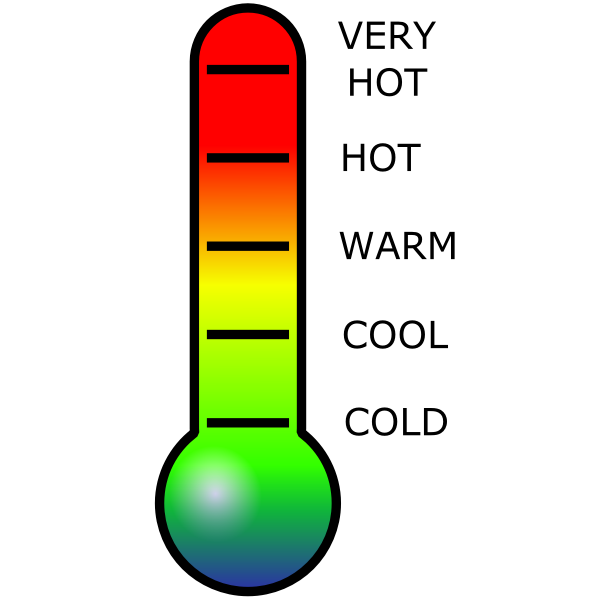
\includegraphics[height=1.25cm]{images/pictograms/temperature}

\includegraphics[height=1.25cm]{images/pictograms/publication}

%%%%%%%%%%%%%%%%%%%%%%%%%%%%%%%%%%%%%%%%%%%%%%%%%%%%%%%%%%%%%%%%%%%%%%%%%%%%%%%%%%%%%%%%%%%%%%%%%%%

\lstinputlisting[language=bash,basicstyle=\small]{python_codes/fieldstone_83/keywords.ascii}

\begin{center}
Code at \url{https://github.com/cedrict/fieldstone/tree/master/python_codes/fieldstone_83}
\end{center}

\par\noindent\rule{\textwidth}{0.4pt}

{\sl This stone was developed in collaboration with Iris van Zelst}. \index{contributors}{I. van Zelst}

\par\noindent\rule{\textwidth}{0.4pt}
%%%%%%%%%%%%%%%%%%%%%%%%%%%%%%%%%%%%%%%%%%%%%%%%%%%%%%%%%%%%%%%%%%%%%%%%%%%%%%%%%%%%%%%%%%%%%%


To accurately study the thermal structure of the oceanic lithosphere, it is important to take 
into account the temperature dependence of thermal parameters such as the thermal conductivity $k$, 
heat capacity $C_p$, and the density $\rho$. Classic (analytical) models, such as the half-space 
cooling model and the plate model, typically ignore this complexity and assume constant parameters.
 
Here, we model the thermal structure of oceanic lithosphere with temperature-dependent 
thermal conductivity, heat capacity, and density according to \textcite{mcjp05} 
and \textcite{rihc18}. 

We use a 2D approach\footnote{This allows us to reuse and adapt an existing 2D code}, 
although there is no lateral variation in the $x$-direction, 
which essentially makes this a 1D model of cooling oceanic lithosphere with time. 
We implement various options for the temperature-dependence of the parameters (including the constant case) 
based on experimental findings and different rock compositions \textcite{pasc77} ({\python model=0}), 
Berman 1988, Berman and Aranovich 1996, Hofmeister 1999, Xu et al., 2004. 
We then compare our results to those of \textcite{rihc18}.

We start from Eq.~(1) of \textcite{mcjp05} (2005):
\[
\frac{\partial}{\partial t}
\left(\rho(T) C_p(T) T \right) = \vec\nabla \cdot \left(k(T) \vec\nabla T \right)
\]
Using a simple Euler scheme we have
\[
\frac{ \left(\rho(T) C_p(T) T \right)^{\color{blue}n} - \left(\rho(T) C_p(T) T \right)^{\color{blue}n-1} }
{\delta t}   = \vec\nabla \cdot (k(T^{\color{blue}n}) \vec\nabla T^{\color{blue}n})
\]
or, simply reorganising the terms: 
\[
\rho(T^{\color{blue}n}) C_p(T^{\color{blue}n}) T^{{\color{blue}n}} - 
\delta t \vec\nabla \cdot (k(T^{\color{blue}n}) \vec\nabla T^n)
= \rho(T^{\color{blue}n-1}) C_p(T^{\color{blue}n-1}) T^{\color{blue}n-1} 
\]
However, since we wish to compute $\vec{T}^{\color{blue} n}$ then 
$\rho(T^{\color{blue}n})$, $C_p(T^{\color{blue}n})$ and $k(T^{\color{blue}n})$ are
not available to us so we resort to using the ones from the previous timestep\footnote{As noted
later we should in fact implement a nonlinear loop and these would become the values 
of the previous iteration.}, or
\[
\rho(T^{\color{blue}n-1}) C_p(T^{\color{blue}n-1}) T^{{\color{blue}n}} - 
\delta t \vec\nabla \cdot (k(T^{\color{blue}n-1}) \vec\nabla T^n)
= \rho(T^{\color{blue}n-1}) C_p(T^{\color{blue}n-1}) T^{\color{blue}n-1} 
\]
We left multiply by a shape function $\bN_i$ and integrate over the whole domain $\Omega$:
\[
\int_\Omega \bN_i \rho(T^{\color{blue}n-1}) C_p(T^{\color{blue}n-1}) T^{{\color{blue}n}} dV-
\delta t \int_\Omega \bN_i \vec\nabla \cdot (k(T^{\color{blue}n-1}) \vec\nabla T^{\color{blue}n}) dV
= 
\int_\Omega \bN_i\rho(T^{\color{blue} n-1}) C_p(T^{\color{blue}n-1}) T^{\color{blue} n-1} dV
\]
Using the basis functions, we can write
\[
T^h(x,y) = \vec{\bN}(x,y) \cdot \vec{T}
\]
where $\vec{T}$ is the vector of nodal temperatures, and this ultimately 
yields\footnote{see Section~\ref{MMM-ss:hte_fem}
for the derivations}
\[
{\bm \M}^{\color{blue}n} \cdot \vec{T}^{\color{blue}n} 
+ \delta t {\bm \K}^{\color{blue}n} \cdot \vec{T}^{\color{blue}n} = \vec{f}^{\color{blue} n-1}
\]
with
\begin{eqnarray}
{\bm \M}^{\color{blue}n} &=& \int_V \rho(T^{\color{blue}n-1}) C_p(T^{\color{blue}n-1}) \vec{\bN}^T \vec{\bN} dV  \nn\\
{\bm \K}^{\color{blue}n} &=& \int_V {\bm B}^T k(T^{\color{blue}n-1}) {\bm B} dV \nn\\
\vec{f}^{\color{blue} n-1} &=& \int_V \vec{\bN}^T \rho(T^{\color{blue} n-1}) C_p(T^{\color{blue}n-1}) dV \nn
\end{eqnarray}
The second term has been integrated by parts (and the surface term disregarded:
Dirichlet boundary conditions top and bottom, and zero heat flux on the sides).

The density is given by Eq.~(9) of \textcite{mcjp05}:
\begin{equation}
\rho(T)=\rho_0 \exp -\left[\alpha_0 (T-273) + \frac{\alpha_1}{2} (T^2-273^2) \right]
\label{eq:f83_1}
\end{equation}
with $\rho_0=3330\si{\kg\per\cubic\meter}$.

The heat capacity is given by Eq.~(10) of \textcite{mcjp05}:
\begin{equation}
C_p(T) = k_0 + k_1 T^{-1/2} + k_3 T^{-3}
\label{eq:f83_2}
\end{equation}
with $k_0=233.18$, $k_1=-1801.6$ and $k_3=-26.794\cdot 10^{7}$ for fosterite and 
$k_0=252$, $k_1=-2013.7$ and $k_3=-6.219\cdot10^{7}$ for fayalite. We assumed that the
molar fraction of fayalite in the mantle is 11\%. 

The heat conductivity is given by Eq.(4) of \textcite{mcjp05}:
\begin{equation}
k(T)=\frac{b}{a+cT} + \sum_{m=0}^3 d_m (T+273)^m
\label{eq:f83_3}
\end{equation}
with $b=5.3$, $c=0.0015$, $d_0=1.753\cdot10^{-2}$, $d_1=-1.0365\cdot10^{-4}$, $d_2=2.2451\cdot10^{-7}$ and 
$d_3=-3.4071\cdot10^{-11}$

Because the coefficients $\rho(T)$, $C_p(T)$ and $k(T)$ depend on the temperature, which is the unknown 
of the PDE, this PDE is highly nonlinear and a dedicated algorithm {\it should} then 
be designed to handle the nonlinearity. For now the code disregards those considerations 
and its structure is identical to the linear equation case. 
We come back to this point hereafter.

Following Richards et al, we run the model for 170~\si{\mega\year}. 
Boundary conditions are $T=0~\si{\celsius}$ 
at the top and $T=1350~\si{\celsius}$ at the bottom. The functions for $k(T)$, $C_p(T)$ and $\rho(T)$
are in a separate file {\python temperature\_dependent\_variables.py}.

In what follows quadratic elements are used (although the code can also be used with linear ones).

%.........................................................................................
\subsection*{A simple case: Constant parameters}

In this case we set $k=3.138~\si{\watt\per\meter\per\kelvin}$, 
$C_p=1171.52~\si{\joule\per\kg\per\kelvin}$ and 
$\rho=3330~\si{\kg\per\cubic\meter}$.

\begin{center}
\includegraphics[width=12cm]{python_codes/fieldstone_83/images/rihc18a}\\
{\captionfont Taken from \textcite{rihc18}. Thermal structure of oceanic lithosphere. 
(a) Simple analytical plate model using the published values reported by \textcite{pasc77}; 
numbered contours = isothermal surfaces plotted in \si{\celsius}; 
green and white circles with error bars = oceanic intraplate and outer rise earthquakes 
from Craig et al. (2014) where small/medium/large circles 
= $M_b < 5.5$, $5.5-6.5$, and $> 6.5$; 
vertical black bars = depth to lithosphere-asthenosphere boundary in the Pacific Ocean
based upon peak variations in azimuthal anisotropy (Burgos et al., 2014); 
dashed box = envelope of depths to lithosphere-asthenosphere boundary for plate 
ages $>100~\si{\mega\year}$ (\textcite{stbe18}); horizontal black dashed line = base of plate model. } 
\end{center}

A word about the time step. It is limited by the value $h^2/\kappa$ where $h$ is the mesh size 
and $\kappa$ is the thermal diffusivity. 
Here, we build the mesh so that $h=1000~\si{\meter}$ and 
$\kappa=k/\rho C_p = 3.138/1171.52 \cdot 3330\simeq 8\cdot 10^{-7}$ (which is very close to the 
typical $10^{-6}$ value), so that the maximum timestep is about 1.24e12s, or about $39421~\si{\year}$. 
We therefore set $\delta t = 10\si{\kilo\year}$. 
Models are run for $170~\si{\mega\year}$, i.e. 17000 time steps!

In essence the code starts by setting the initial temperature to the bottom value and 
then proceeds to solve the equation in time, thereby producing a profile that starts on the 
left of the figure above and ends on the right side of it.

\begin{center}
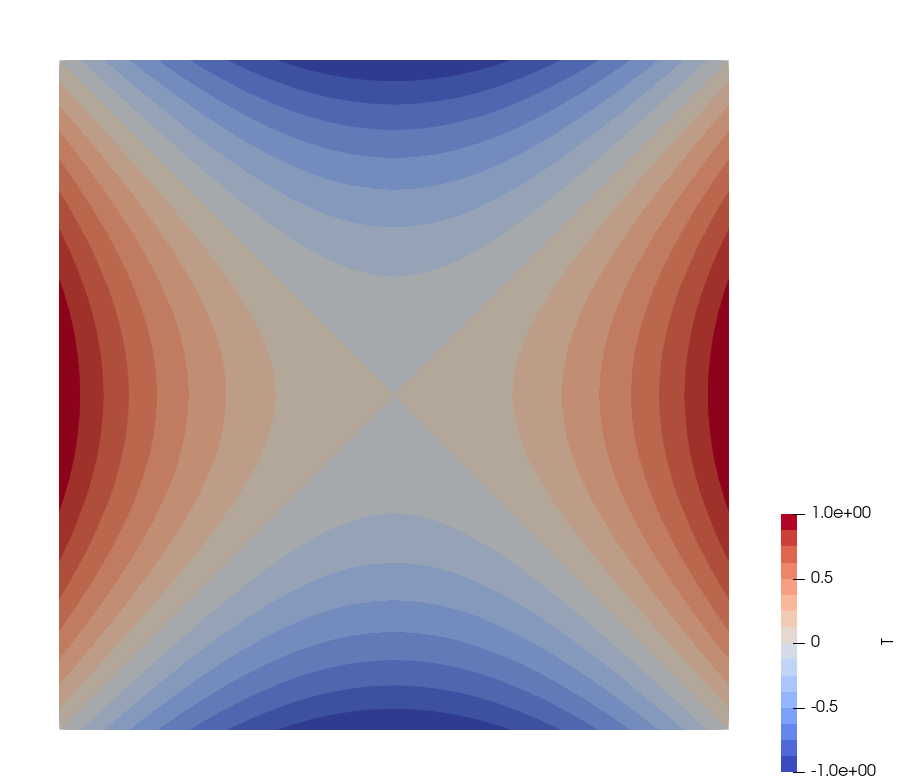
\includegraphics[width=8cm]{python_codes/fieldstone_83/results_model1/T}
\includegraphics[width=7cm]{python_codes/fieldstone_83/results_model1/comparison}\\
{\captionfont Left: Isocontours every 100$\si{\celsius}$ between $0\si{\celsius}$ and $1300\si{\celsius}$. 
Right: our results (green lines) super-imposed on those of \textcite{rihc18}.}
\end{center}

\begin{center}
\includegraphics[width=10cm]{python_codes/fieldstone_83/results_model1/Tprofiles}\\
{\captionfont Temperature profile evolution as a function of time. The analytical solution
is plotted at $t=20~\si{\mega\year}$ and it agrees with out numerical solution, 
which thereby benchmarks our code.} 
\end{center}


%....................................................................
\subsection*{T-dependent parameters a la McKenzie et al (2015)}

\begin{center}
\includegraphics[width=12cm]{python_codes/fieldstone_83/images/rihc18b}\\
{\captionfont Same for the purely temperature-dependent plate model using parameter values from
\textcite{mcjp05}. Note that the initial temperature on the left seems to have changed?}
\end{center}


\begin{center}
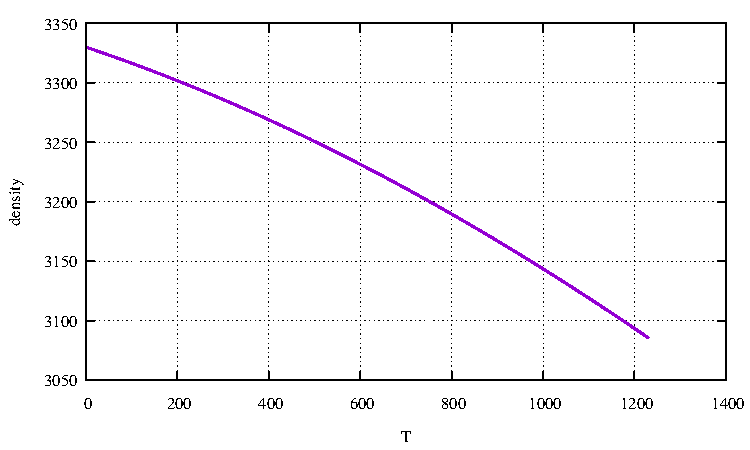
\includegraphics[width=7cm]{python_codes/fieldstone_83/results_model2/rho.pdf}
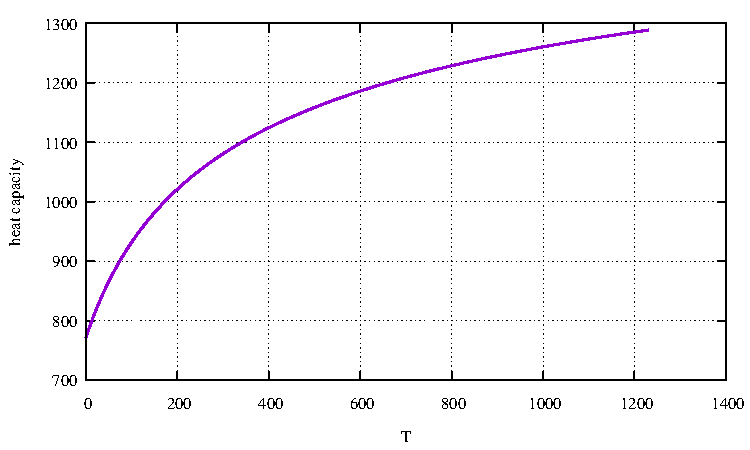
\includegraphics[width=7cm]{python_codes/fieldstone_83/results_model2/hcapa.pdf}\\
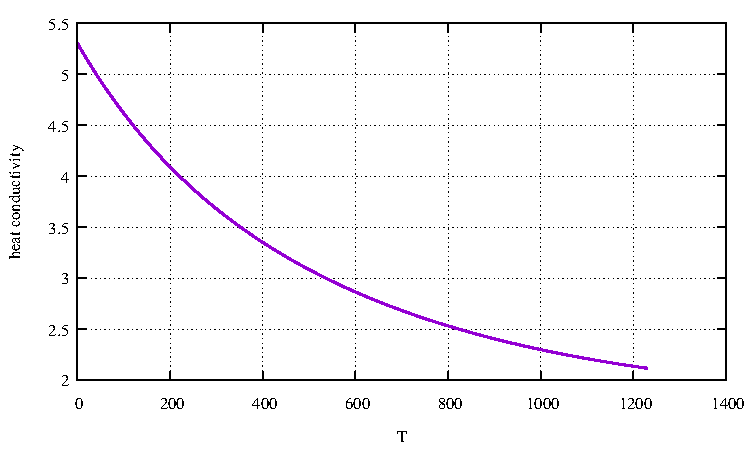
\includegraphics[width=7cm]{python_codes/fieldstone_83/results_model2/hcond.pdf}
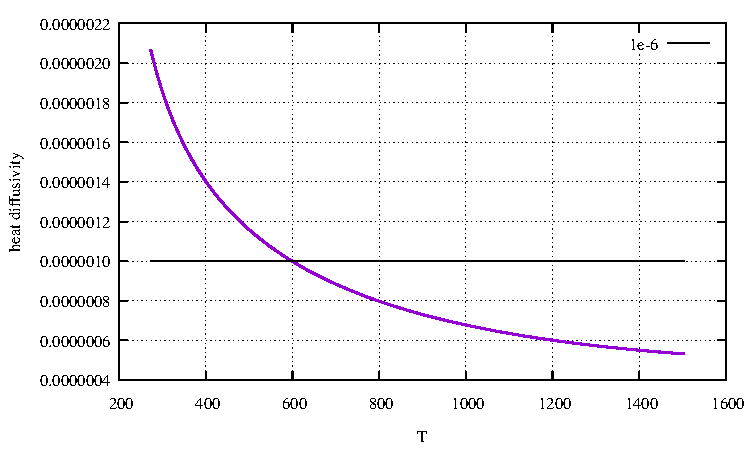
\includegraphics[width=7cm]{python_codes/fieldstone_83/results_model2/kappa.pdf}\\
{\captionfont Density, heat capacity and heat conductivity as obtained from Eqs.~\eqref{eq:f83_1}, 
\eqref{eq:f83_2}, and \eqref{eq:f83_3}, and heat diffusivity $\kappa$.}
\end{center}

Looking at the heat diffusivity values, we see that these are at most twice as large 
as above. As such the value of $\delta t = 10\si{\kilo\year}$ is still warranted.

\begin{center}
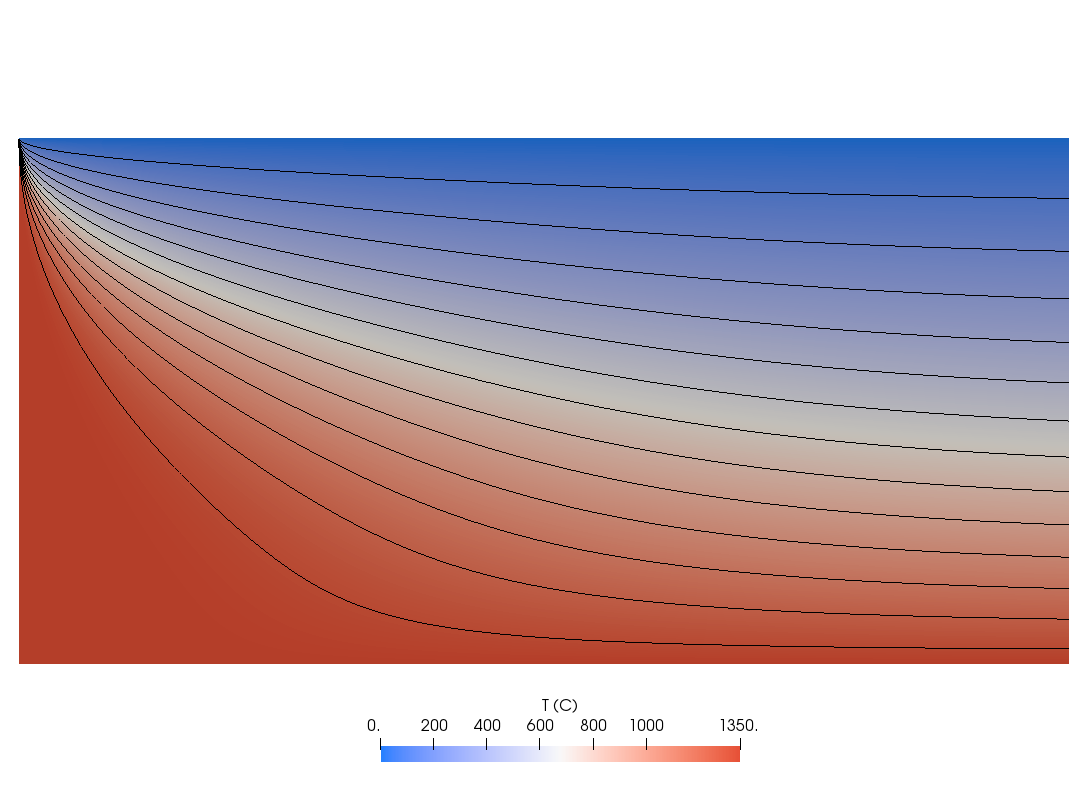
\includegraphics[width=8cm]{python_codes/fieldstone_83/results_model2/T}
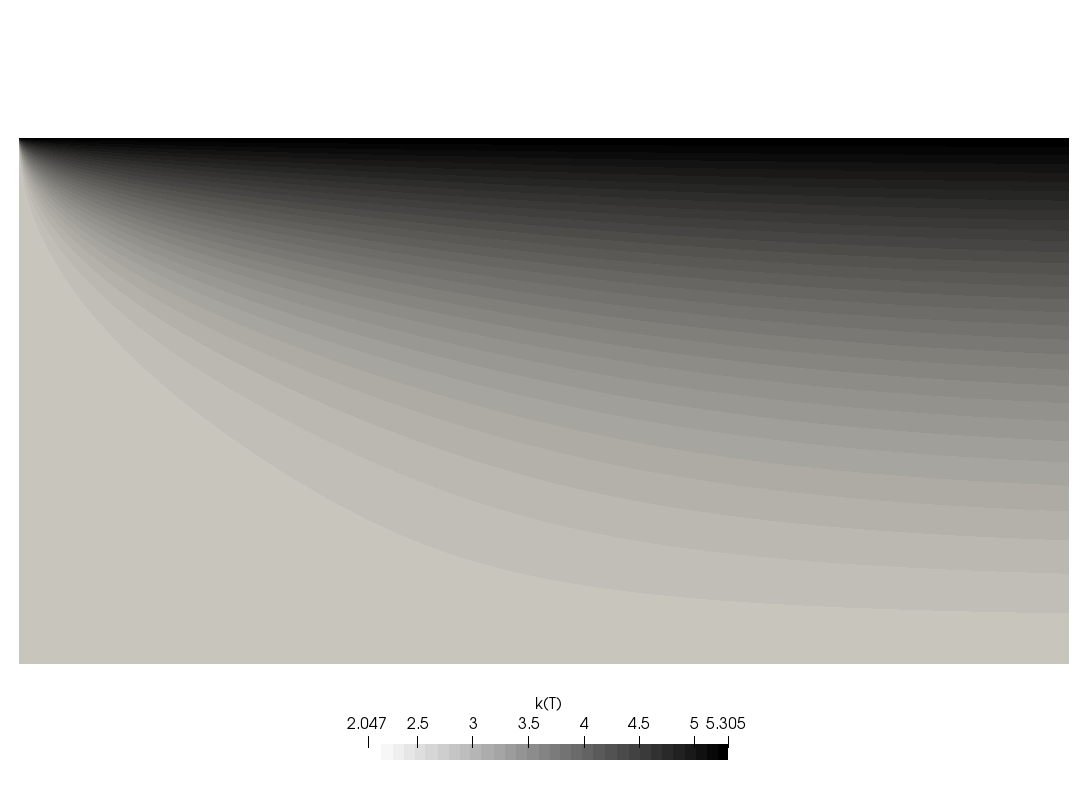
\includegraphics[width=8cm]{python_codes/fieldstone_83/results_model2/k}\\
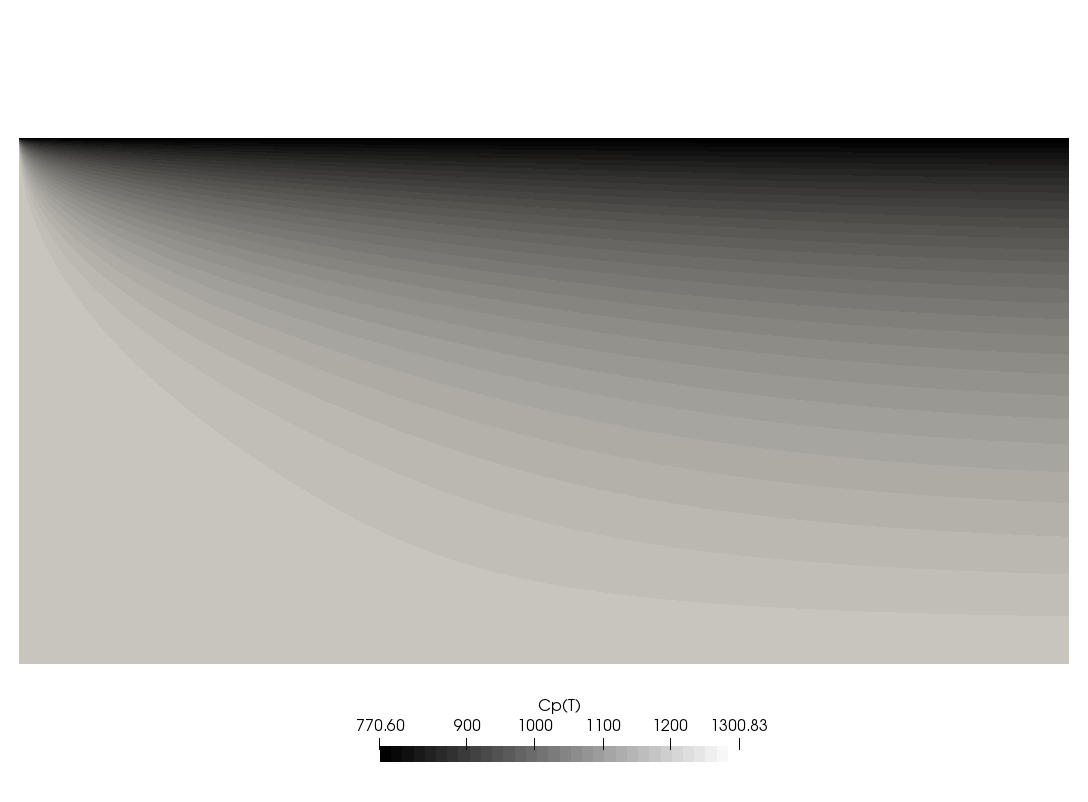
\includegraphics[width=8cm]{python_codes/fieldstone_83/results_model2/Cp}
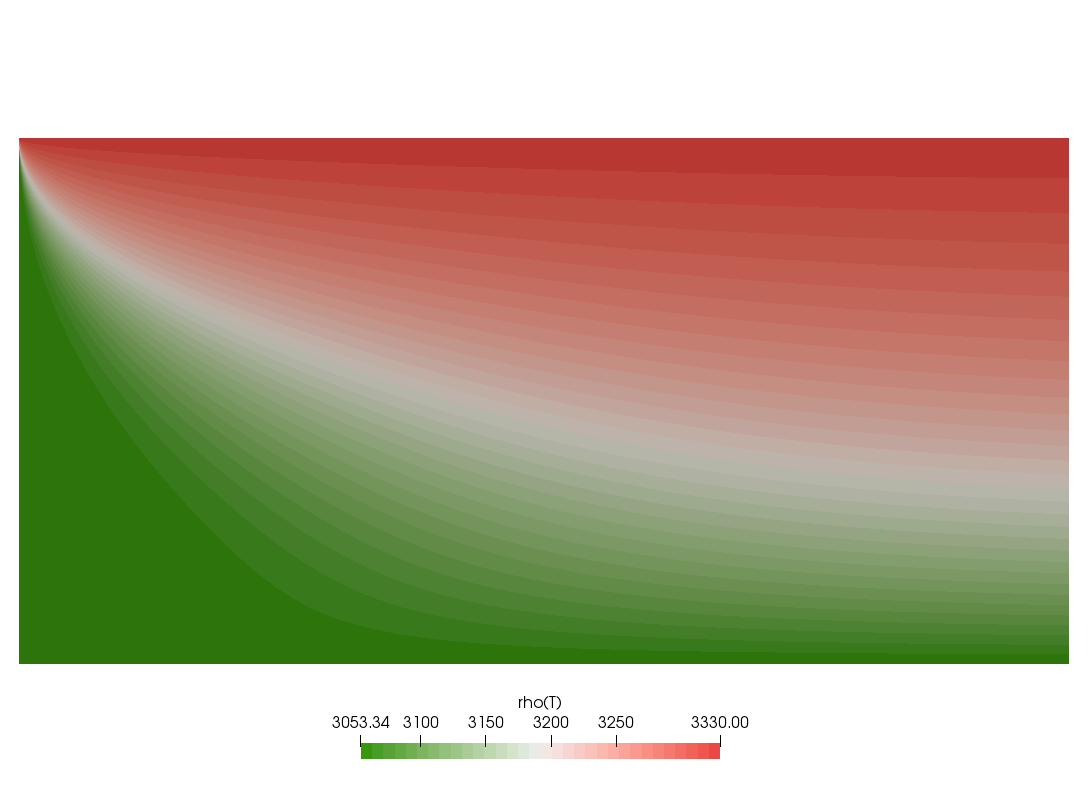
\includegraphics[width=8cm]{python_codes/fieldstone_83/results_model2/rho.png}\\
{\captionfont Temperature, heat conductivity, heat capacity and density profiles
as a function of time.}
\end{center}

\begin{center}
\includegraphics[width=10cm]{python_codes/fieldstone_83/results_model2/Tprofiles}\\
{\captionfont Temperature profile evolution. In this case there is obviously no analytical solution.}
\end{center}

Although there is no appropriate algorithm to deal with the nonlinear character of the 
equation, we can carry out a simple test by changing the timestep to 5,10,20kr
and after 20Myr we find that temperatures do not differ by more than 0.2K. 
It does not replace a proper nonlinear Picard algorithm but this simple check 
allows us to assess that when using extremely small time steps (akin to in fact doing many
nonlinear iterations per larger time step - cost wise), the solution does not change 
significantly.




